\documentclass[12pt]{article}

% --------------------------------------------------------
% FONTS & ENCODING
% --------------------------------------------------------
\usepackage[T1]{fontenc}
\usepackage[utf8]{inputenc}
\usepackage{lmodern}

% --------------------------------------------------------
% PAGE SETUP
% --------------------------------------------------------
\usepackage[margin=1in]{geometry}
\usepackage{ragged2e}
\usepackage{graphicx}
\usepackage{float}
\usepackage{hyperref}
\hypersetup{
  colorlinks=true,
  linkcolor=blue!60!black,
  urlcolor=blue!60!black
}

\setlength{\parskip}{8pt}
\setlength{\parindent}{0pt}

% --------------------------------------------------------
% COLORS & SECTION STYLING
% --------------------------------------------------------
\usepackage{xcolor}
\usepackage{sectsty}
\usepackage{titlesec}

\definecolor{mainDark}{HTML}{2C3E50}
\definecolor{awsColor}{HTML}{F8C471}
\definecolor{localColor}{HTML}{82E0AA}
\definecolor{userColor}{HTML}{85C1E9}
\definecolor{boxBg}{HTML}{F8F9FA}

\sectionfont{\color{mainDark}\huge}
\subsectionfont{\color{mainDark}\Large}
\titlespacing*{\section}{0pt}{1em}{0.5em}
\titlespacing*{\subsection}{0pt}{0.8em}{0.3em}

% --------------------------------------------------------
% CODE LISTINGS
% --------------------------------------------------------
\usepackage{minted}
\usemintedstyle{friendly}

% --------------------------------------------------------
% TIKZ DIAGRAMS
% --------------------------------------------------------
\usepackage{tikz}
\usetikzlibrary{shapes,arrows,positioning,calc,arrows.meta,shapes.misc}

% Styles for color-coded boxes
\tikzset{
  userBox/.style={
    rectangle,
    rounded corners,
    draw=mainDark,
    fill=userColor!40,
    text width=3cm,
    minimum height=1.2cm,
    align=center
 },
  localBox/.style={
    rectangle,
    rounded corners,
    draw=mainDark,
    fill=localColor!40,
    text width=3cm,
    minimum height=1.2cm,
    align=center
 },
  awsBox/.style={
    rectangle,
    rounded corners,
    draw=mainDark,
    fill=awsColor!40,
    text width=3cm,
    minimum height=1.2cm,
    align=center
 },
  arrowLine/.style={
    -{Latex[length=3mm,width=2mm]},
    thick,
    color=mainDark
 }
}

% --------------------------------------------------------
% TITLE
% --------------------------------------------------------
\title{
    \vspace{-2cm}
    \textbf{\color{mainDark}\Huge AWS: A Simple, Visual Guide}\\
    \vspace{0.2cm}
    \large \textit{With Plain Definitions, Diagrams, and Detailed Comparisons}
}
\author{}
\date{}

\begin{document}
\maketitle
\vspace{-1cm}

% --------------------------------------------------------
% INTRO
% --------------------------------------------------------
\section*{Introduction}
\justifying
\textbf{Amazon Web Services (AWS)} provides on-demand infrastructure and services so you don't have to buy or maintain physical servers. You pay only for what you use, and you can scale up or down easily. This document explains \textit{how AWS services interact}, \textit{how data flows in multiple directions}, and \textit{the differences/similarities between storage/database services like S3, RDS, DynamoDB, EBS}, and others. We'll keep definitions simple and include helpful diagrams.

\begin{center}
    \resizebox{0.7\textwidth}{!}{
        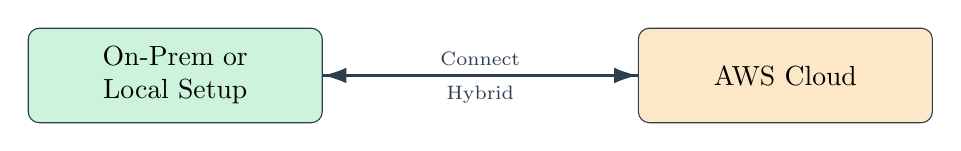
\begin{tikzpicture}[node distance=4cm]
            \node[localBox, text width=3.5cm] (local) {On-Prem or\\Local Setup};
            \node[awsBox, text width=3.5cm, right=4cm of local] (cloud) {AWS Cloud};

            \draw[arrowLine] (local) -- node[above]{\scriptsize Connect} (cloud);
            \draw[arrowLine] (cloud) -- node[below]{\scriptsize Hybrid} (local);
        \end{tikzpicture}
    }
\end{center}

\clearpage

% --------------------------------------------------------
% 1. KEY TERMS & DEFINITIONS
% --------------------------------------------------------
\section{Key Terms \& Definitions (Quick Glossary)}
\justifying
Here are concise definitions for core AWS terms used throughout this guide. Check the diagrams to visualize how they interact.

\subsection*{Region}
A geographical area (e.g., \texttt{us-east-1} or \texttt{eu-west-1}). Each region hosts multiple data centers.

\subsection*{Availability Zone (AZ)}
One or more data centers in a region. Deploying resources across AZs can increase resilience.

\subsection*{EC2 (Elastic Compute Cloud)}
Virtual machines in AWS. You choose the OS, apps, and scale as needed. AWS manages the physical servers.

\subsection*{Lambda (Serverless)}
Upload code, and AWS runs it whenever an event triggers it (e.g., S3 file upload). No need to manage servers.

\subsection*{S3 (Simple Storage Service)}
Object storage: store files, images, backups, or logs in \textit{buckets}. Highly durable and globally accessible.

\subsection*{EBS (Elastic Block Store)}
Block storage for \textbf{EC2} instances, like a virtual hard drive you attach to your EC2 VM.

\subsection*{RDS (Relational Database Service)}
Managed SQL database (MySQL, PostgreSQL, etc.). AWS handles patches, backups, and scaling up to a point.

\subsection*{DynamoDB}
A NoSQL key-value database. Can handle massive throughput and scales horizontally.

\subsection*{CloudFront}
A Content Delivery Network (CDN) that caches or delivers content from edge locations near the user.

\subsection*{Load Balancer (ELB)}
Distributes incoming traffic among multiple EC2 servers or containers so no single server is overwhelmed.

\subsection*{API Gateway}
Front-end for your REST or WebSocket APIs. Often used with \textbf{Lambda} or \textbf{EC2} to route external calls.

\subsection*{SNS (Simple Notification Service)}
Sends messages to subscribers (e.g., email, text, or AWS services) when certain events happen.

\subsection*{EventBridge}
An advanced event bus system that can route events from multiple AWS sources (like S3, EC2) or external apps to your services.

\subsection*{Kinesis}
A service for ingesting and processing large streams of data in real time (e.g., logs, sensor data).

\subsection*{Redshift}
A data warehouse solution for large-scale analytical queries. Good for big data (SQL-based).

\subsection*{Athena}
Run SQL queries on files stored in \textbf{S3} with no need to manage a database cluster.

\subsection*{SageMaker}
AWS platform to train and deploy machine learning models without manually setting up servers.

\subsection*{ECS/EKS}
Containers on AWS. \textbf{ECS} is Amazon's own container orchestration, \textbf{EKS} is AWS-managed Kubernetes.

\subsection*{Route 53}
AWS's Domain Name System (DNS) service. It can route users to different Regions or services.

\subsection*{IoT}
AWS IoT services let physical devices (sensors, microcontrollers) send/receive data in the cloud.

\subsection*{VPN / DirectConnect}
Methods to link your on-premises data center to AWS, creating a \textbf{hybrid} environment.

\clearpage

% --------------------------------------------------------
% 2. HOW SERVICES INTERACT (HIGH-LEVEL)
% --------------------------------------------------------
\section{How AWS Services Interact (High-Level)}

\begin{center}
    \resizebox{0.9\textwidth}{!}{
        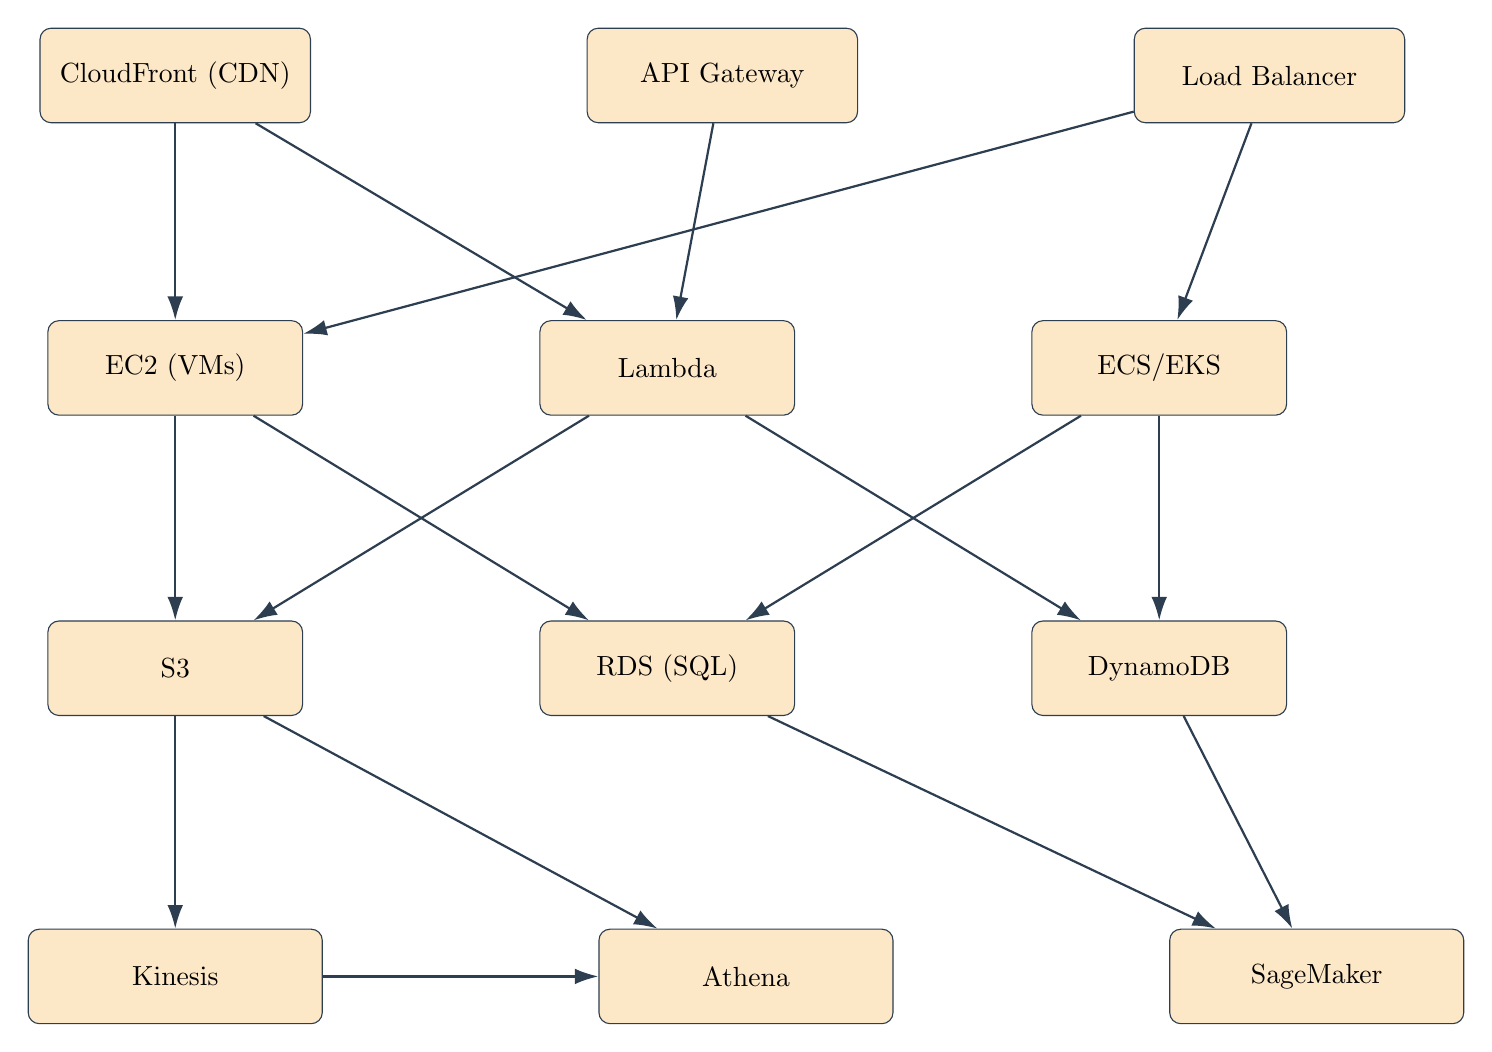
\begin{tikzpicture}[node distance=2.5cm]

            % Top row: "Frontend"
            \node[awsBox, text width=3.2cm] (cloudfront) {CloudFront (CDN)};
            \node[awsBox, text width=3.2cm, right=3.5cm of cloudfront] (api) {API Gateway};
            \node[awsBox, text width=3.2cm, right=3.5cm of api] (elb) {Load Balancer};

            % Middle row: "Compute"
            \node[awsBox, text width=3cm, below=2.5cm of cloudfront] (ec2) {EC2 (VMs)};
            \node[awsBox, text width=3cm, right=3cm of ec2] (lambda) {Lambda};
            \node[awsBox, text width=3cm, right=3cm of lambda] (containers) {ECS/EKS};

            % Storage / DB
            \node[awsBox, text width=3cm, below=2.6cm of ec2] (s3) {S3};
            \node[awsBox, text width=3cm, right=3cm of s3] (rds) {RDS (SQL)};
            \node[awsBox, text width=3cm, right=3cm of rds] (dynamo) {DynamoDB};

            % Lower row: "Analytics / ML"
            \node[awsBox, text width=3.5cm, below=2.7cm of s3] (kinesis) {Kinesis};
            \node[awsBox, text width=3.5cm, right=3.5cm of kinesis] (athena) {Athena};
            \node[awsBox, text width=3.5cm, right=3.5cm of athena] (sagemaker) {SageMaker};

            % Arrows top to middle
            \draw[arrowLine] (cloudfront) -- (ec2);
            \draw[arrowLine] (cloudfront) -- (lambda);
            \draw[arrowLine] (api) -- (lambda);
            \draw[arrowLine] (elb) -- (ec2);
            \draw[arrowLine] (elb) -- (containers);

            % Middle to storage
            \draw[arrowLine] (ec2) -- (s3);
            \draw[arrowLine] (ec2) -- (rds);
            \draw[arrowLine] (lambda) -- (s3);
            \draw[arrowLine] (lambda) -- (dynamo);
            \draw[arrowLine] (containers) -- (rds);
            \draw[arrowLine] (containers) -- (dynamo);

            % Storage to analytics
            \draw[arrowLine] (s3) -- (kinesis);
            \draw[arrowLine] (kinesis) -- (athena);
            \draw[arrowLine] (dynamo) -- (sagemaker);
            \draw[arrowLine] (rds) -- (sagemaker);
            \draw[arrowLine] (s3) -- (athena);

        \end{tikzpicture}
    }
\end{center}

\noindent
\textbf{Observations:}
\begin{itemize}
    \item Services like \textbf{CloudFront}, \textbf{API Gateway}, or \textbf{ELB} handle incoming traffic.
    \item \textbf{EC2}, \textbf{Lambda}, or \textbf{ECS/EKS} do the compute work.
    \item \textbf{S3}, \textbf{RDS}, and \textbf{DynamoDB} provide storage or database solutions.
    \item Tools like \textbf{Kinesis}, \textbf{Athena}, and \textbf{SageMaker} handle analytics or ML tasks.
\end{itemize}

\clearpage

% --------------------------------------------------------
% 3. COMPARING S3, EBS, RDS, DYNAMODB, ETC.
% --------------------------------------------------------
\section{AWS Storage \& Database Comparisons}

AWS has \textbf{multiple ways to store data}. Each one fits different use cases.

\subsection*{3.1. S3 vs. EBS vs. EFS (for completeness)}
\begin{itemize}
    \item \textbf{S3 (Object Storage)}:
          \begin{itemize}
              \item Store files in buckets.
              \item Access via HTTP/HTTPS.
              \item Good for images, backups, static websites.
              \item Not a traditional filesystem. You get objects, not directories in the same sense.
          \end{itemize}
    \item \textbf{EBS (Block Storage)}:
          \begin{itemize}
              \item Attaches to \textbf{one} EC2 instance like a hard drive.
              \item You can format it with a filesystem (e.g., ext4) and mount it in your VM.
              \item Good for running databases on a single server or storing OS-level data.
          \end{itemize}
    \item \textbf{EFS (Elastic File System)}:
          \begin{itemize}
              \item Network file system that can be shared by multiple EC2 instances at once.
              \item If you need standard POSIX filesystem features across multiple servers.
          \end{itemize}
\end{itemize}

\subsection*{3.2. RDS (SQL) vs. DynamoDB (NoSQL)}
\begin{itemize}
    \item \textbf{RDS (Relational Database Service)}:
          \begin{itemize}
              \item SQL-based (MySQL, PostgreSQL, etc.).
              \item Tables with columns and rows. Great for structured queries and relationships.
              \item AWS manages backups, patches, scaling up to a limit. For read scaling, you can add read replicas.
          \end{itemize}
    \item \textbf{DynamoDB (NoSQL)}:
          \begin{itemize}
              \item Key-value or document-based.
              \item Scales horizontally. You can handle extremely high request rates with auto-scaling.
              \item Great for simple queries on large amounts of data.
              \item Doesn’t support complex SQL joins or relationships well.
          \end{itemize}
\end{itemize}

\begin{center}
    \resizebox{0.95\textwidth}{!}{
        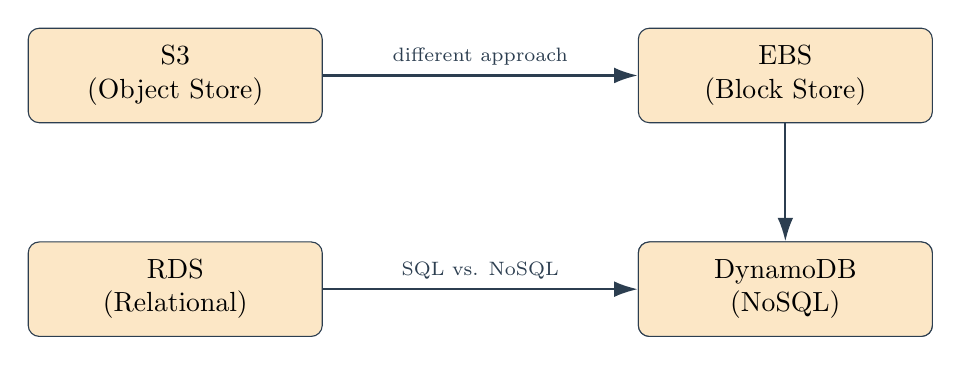
\begin{tikzpicture}[node distance=4cm]
            % S3 box
            \node[awsBox, text width=3.5cm] (s3) {S3\\(Object Store)};
            % EBS box
            \node[awsBox, text width=3.5cm, right=4cm of s3] (ebs) {EBS\\(Block Store)};
            % EFS box (optional)
            \node[awsBox, text width=3.5cm, below=1.5cm of ebs] (efs) {EFS\\(Shared File)};

            \draw[arrowLine] (s3) -- node[above]{\scriptsize different approach} (ebs);
            \draw[arrowLine] (ebs) -- (efs);

            % RDS box
            \node[awsBox, text width=3.5cm, below=1.5cm of s3] (rds) {RDS\\(Relational)};
            \node[awsBox, text width=3.5cm, right=4cm of rds] (ddb) {DynamoDB\\(NoSQL)};

            \draw[arrowLine] (rds) -- node[above]{\scriptsize SQL vs. NoSQL} (ddb);
        \end{tikzpicture}
    }
\end{center}

\noindent
\textbf{Basic rule of thumb}:
\begin{itemize}
    \item If you want to store \textit{files} or \textit{objects} (like images, PDFs), \textbf{S3} is best.
    \item If you need a \textbf{disk} attached to an EC2 instance, use \textbf{EBS}.
    \item If multiple servers need to share a network filesystem, use \textbf{EFS}.
    \item If you want a \textbf{SQL} database, choose \textbf{RDS}.
    \item If you want a \textbf{NoSQL} (key-value) database that scales big, pick \textbf{DynamoDB}.
\end{itemize}

\clearpage

% --------------------------------------------------------
% 4. EXAMPLE OF INTERACTIONS AMONG THESE STORES
% --------------------------------------------------------
\section{Interactions Among S3, EBS, RDS, and DynamoDB}

\subsection*{4.1 Architecture Diagram}
\begin{center}
    \resizebox{0.85\textwidth}{!}{
        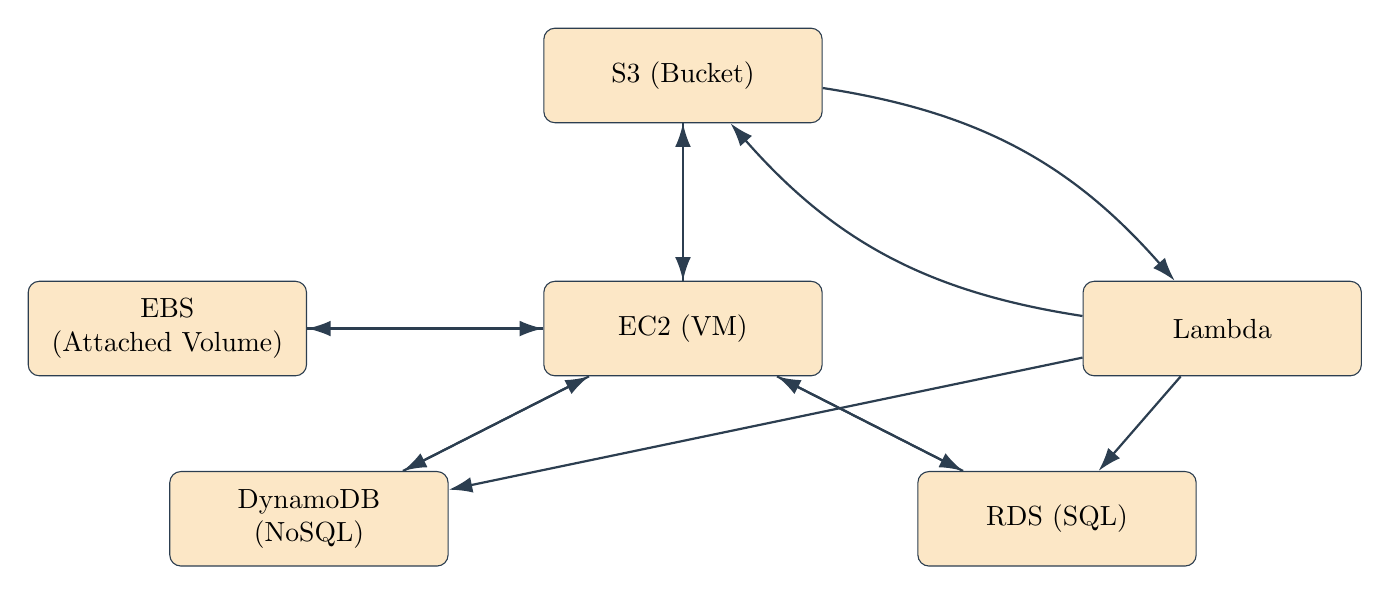
\begin{tikzpicture}[node distance=3cm]

            % EC2 in the middle
            \node[awsBox, text width=3.3cm] (ec2) {EC2 (VM)};

            % EBS to the left
            \node[awsBox, text width=3.3cm, left=3cm of ec2] (ebs) {EBS\\(Attached Volume)};
            \draw[arrowLine] (ec2) -- (ebs);
            \draw[arrowLine] (ebs) -- (ec2);

            % S3 on top
            \node[awsBox, text width=3.3cm, above=2cm of ec2] (s3) {S3 (Bucket)};
            \draw[arrowLine] (ec2) -- (s3);
            \draw[arrowLine] (s3) -- (ec2);

            % RDS on bottom
            \node[awsBox, text width=3.3cm, below right=1.7cm of ec2] (rds) {RDS (SQL)};
            \draw[arrowLine] (ec2) -- (rds);
            \draw[arrowLine] (rds) -- (ec2);

            % Dynamo on bottom left
            \node[awsBox, text width=3.3cm, below left=1.7cm of ec2] (ddb) {DynamoDB (NoSQL)};
            \draw[arrowLine] (ec2) -- (ddb);
            \draw[arrowLine] (ddb) -- (ec2);

            % Possibly show S3 <-> Lambda or something
            \node[awsBox, text width=3.3cm, right=3.3cm of ec2] (lambda) {Lambda};
            \draw[arrowLine] (s3) to[bend left=20] (lambda);
            \draw[arrowLine] (lambda) to[bend left=20] (s3);
            \draw[arrowLine] (lambda) -- (rds);
            \draw[arrowLine] (lambda) -- (ddb);

        \end{tikzpicture}
    }
\end{center}

\noindent
\textbf{Explanations}:
\begin{itemize}
    \item \textbf{EBS} is a virtual disk that the EC2 instance uses like a normal hard drive (storing OS files, logs, etc.).
    \item \textbf{S3} can store large objects or backups for the EC2 instance. The instance can upload or download files to S3.
    \item \textbf{RDS} might store relational (SQL) data for the application running on EC2.
    \item \textbf{DynamoDB} might store NoSQL data if the app needs a key-value store for certain high-scale operations.
    \item \textbf{Lambda} can be triggered by changes in S3 or read/writes to RDS or DynamoDB too, adding serverless workflows.
\end{itemize}

\subsection*{4.2 Differences in Data Access Patterns}
\begin{itemize}
    \item \textbf{EBS:} Accessed only by the EC2 instance it's attached to (unless you do specialized multi-attach). Speaks like a normal drive: ext4, NTFS, etc.
    \item \textbf{S3:} Accessed by \texttt{HTTP/HTTPS}, can be from EC2, Lambda, or even the public internet if you allow it.
    \item \textbf{RDS:} Accessed via SQL queries (e.g., MySQL protocol). Typically from your application.
    \item \textbf{DynamoDB:} Accessed via AWS SDK or APIs. You do read/write operations with a primary key.
\end{itemize}

\clearpage

% --------------------------------------------------------
% 5. SAMPLE LAMBDA CODE (RECAP)
% --------------------------------------------------------
\section{Sample Lambda Code (Recap)}
\justifying
Here’s a simple AWS Lambda function in Python. Notice naming style: \textbf{PascalCase} for functions, \textbf{camelCase} for variables, and \textbf{MACRO\_CASE} for constants.

\begin{minted}[fontsize=\small, frame=single]{python}
def ProcessFile(event, context):
    # event: Contains details about what triggered this function (e.g., S3 upload).
    # context: AWS environment info (e.g., memory, request ID).

    fileKey = event["Records"][0]["s3"]["object"]["key"]
    print("Processing file:", fileKey)

    MACRO_CONSTANT = 100
    processedResult = f"File {fileKey} processed with constant {MACRO_CONSTANT}"

    # Possibly store in S3, or update RDS / DynamoDB
    return {
        "statusCode": 200,
        "body": processedResult
    }
\end{minted}

\clearpage

% --------------------------------------------------------
% 6. USE CASES WITH MULTI-DIRECTION FLOWS
% --------------------------------------------------------
\section{Use Cases (Multi-Directional Flows)}

\subsection*{6.1 Serverless File Processing with DynamoDB Logging}
\begin{center}
    \resizebox{0.9\textwidth}{!}{
        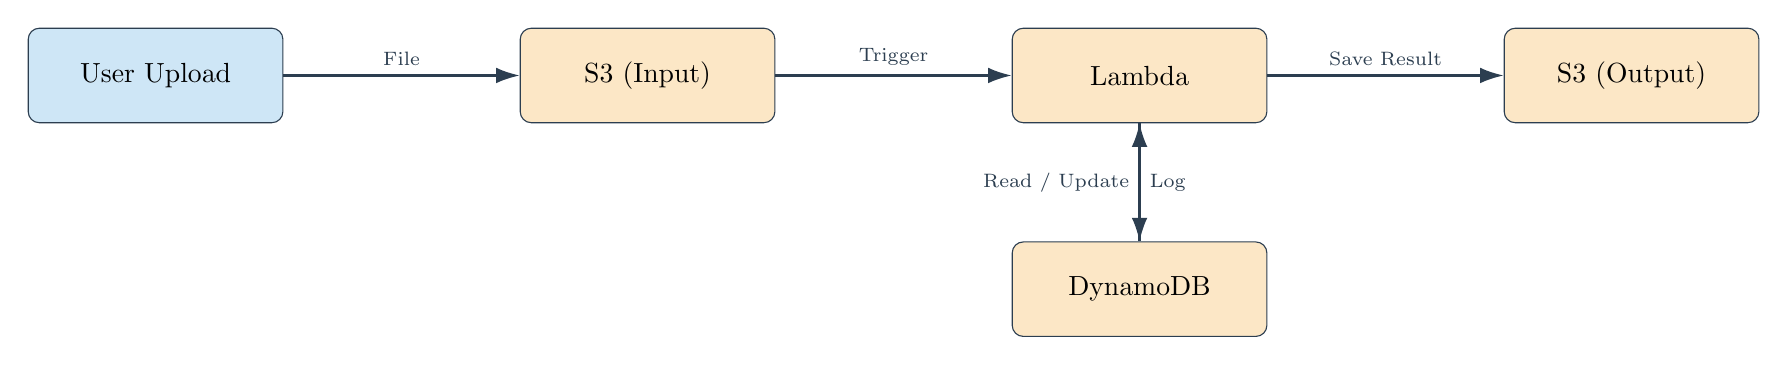
\begin{tikzpicture}[node distance=3cm]
            \node[userBox] (upload) {User Upload};
            \node[awsBox, right=3cm of upload] (s3in) {S3 (Input)};
            \node[awsBox, right=3cm of s3in] (lambda) {Lambda};
            \node[awsBox, right=3cm of lambda] (s3out) {S3 (Output)};
            \node[awsBox, below=1.5cm of lambda, text width=3cm] (ddb) {DynamoDB};

            \draw[arrowLine] (upload) -- node[above]{\scriptsize File} (s3in);
            \draw[arrowLine] (s3in) -- node[above]{\scriptsize Trigger} (lambda);
            \draw[arrowLine] (lambda) -- node[above]{\scriptsize Save Result} (s3out);

            % Additional arrow to Dynamo
            \draw[arrowLine] (lambda) -- node[right]{\scriptsize Log} (ddb);
            \draw[arrowLine] (ddb) -- node[left]{\scriptsize Read / Update} (lambda);
        \end{tikzpicture}
    }
\end{center}
\noindent
\textbf{Flow:}
1. User uploads to S3.
2. Lambda processes the file.
3. Output is saved in another S3 bucket.
4. Lambda also logs metadata to DynamoDB (key-value store).

\subsection*{6.2 A Hybrid Database Approach}
\begin{center}
    \resizebox{0.95\textwidth}{!}{
        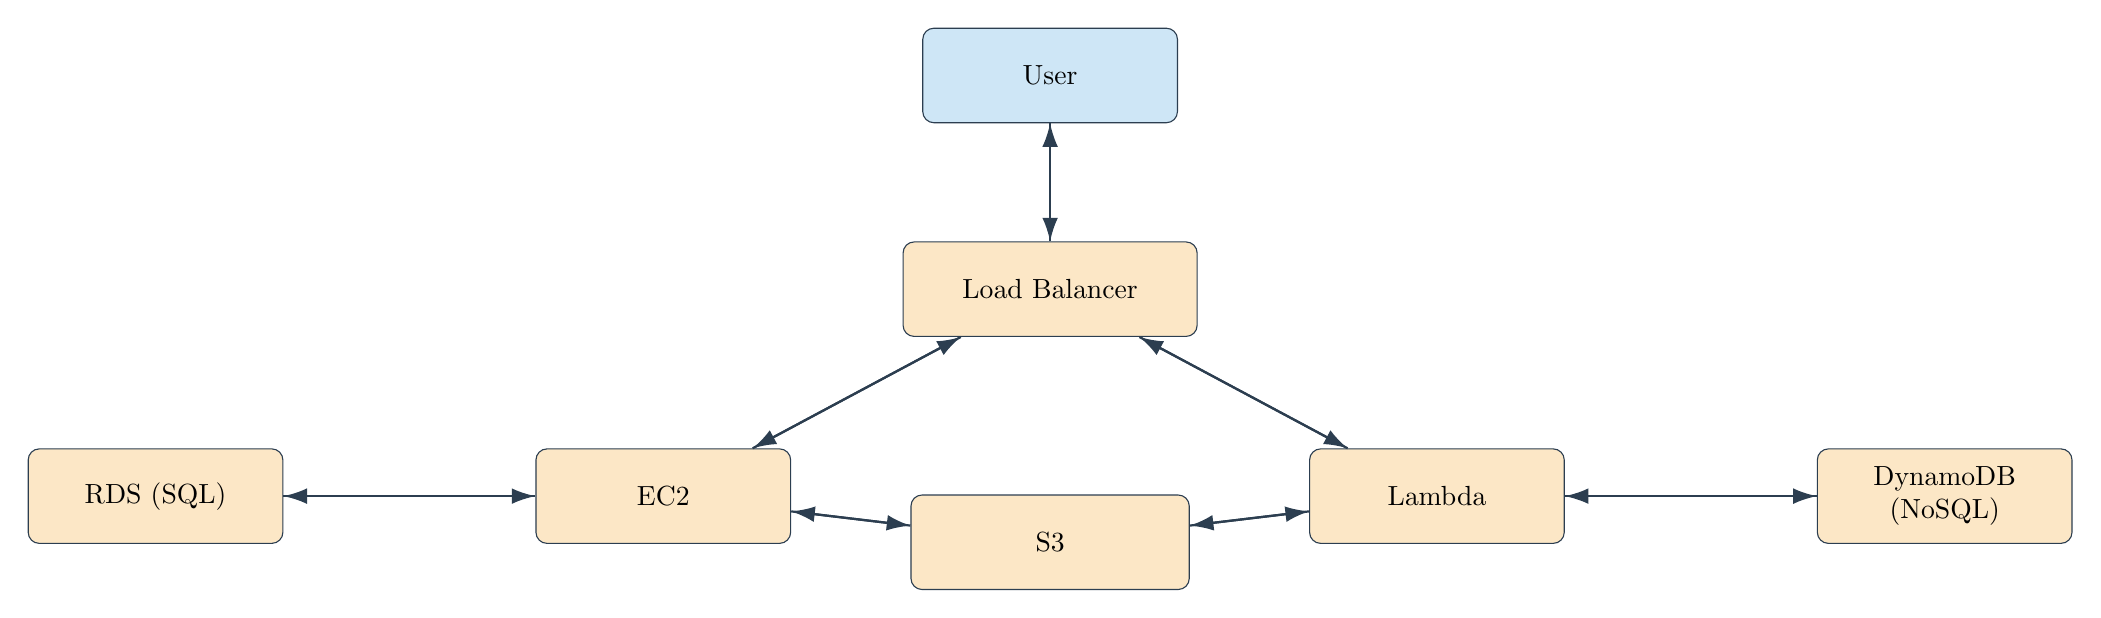
\begin{tikzpicture}[node distance=3cm]
            \node[userBox] (user) {User};

            \node[awsBox, below=1.5cm of user, text width=3.5cm] (elb) {Load Balancer};
            \draw[arrowLine] (user) -- (elb);
            \draw[arrowLine] (elb) -- (user);

            \node[awsBox, below left=2cm of elb] (ec2) {EC2};
            \node[awsBox, below right=2cm of elb] (lambda) {Lambda};

            \draw[arrowLine] (elb) -- (ec2);
            \draw[arrowLine] (ec2) -- (elb);
            \draw[arrowLine] (elb) -- (lambda);
            \draw[arrowLine] (lambda) -- (elb);

            \node[awsBox, left=3.2cm of ec2] (rds) {RDS (SQL)};
            \node[awsBox, right=3.2cm of lambda] (ddb) {DynamoDB (NoSQL)};

            \draw[arrowLine] (ec2) -- (rds);
            \draw[arrowLine] (rds) -- (ec2);

            \draw[arrowLine] (lambda) -- (ddb);
            \draw[arrowLine] (ddb) -- (lambda);

            % Possibly S3 in the middle for file storage
            \node[awsBox, below=2cm of elb, text width=3.3cm] (s3) {S3};
            \draw[arrowLine] (ec2) -- (s3);
            \draw[arrowLine] (lambda) -- (s3);
            \draw[arrowLine] (s3) -- (ec2);
            \draw[arrowLine] (s3) -- (lambda);

        \end{tikzpicture}
    }
\end{center}
\noindent
\textbf{Flow:}
1. Some data is stored in RDS for \textbf{transactional} or \textbf{relational} needs.
2. Some data is in DynamoDB for \textbf{high throughput} or \textbf{simple key-value} lookups.
3. S3 holds files or static assets.
4. Both \textbf{EC2} and \textbf{Lambda} can read from or write to any of these stores.

\clearpage

% --------------------------------------------------------
% 7. CONCLUSION
% --------------------------------------------------------
\section*{Conclusion}
\justifying
AWS provides many ways to store and manage data (\textbf{S3}, \textbf{EBS}, \textbf{RDS}, \textbf{DynamoDB}, etc.), each suited to different use cases. By mixing these services and letting data flow in multiple directions, you can build flexible, scalable architectures.
\bigskip

\textbf{Key Points:}
\begin{itemize}
    \item \textbf{S3} is object storage for files, \textbf{EBS} is block storage for EC2 volumes, \textbf{RDS} handles SQL, and \textbf{DynamoDB} is NoSQL.
    \item Compute can be \textbf{EC2} (full server) or \textbf{Lambda} (serverless). Both can talk to the same storage or database.
    \item Frontend services like \textbf{CloudFront}, \textbf{API Gateway}, and \textbf{ELB} route user traffic.
    \item Multi-directional flows are common: a Lambda might read from S3, write to DynamoDB, then trigger an event for more processing.
\end{itemize}

\noindent
\textbf{Next Steps}:
\begin{itemize}
    \item Sign up for the \textbf{AWS Free Tier} to try building your own environment.
    \item Read the \href{https://docs.aws.amazon.com}{\textbf{AWS Documentation}} for deeper tutorials on each service.
    \item Experiment with a small project (e.g., a static site on S3 + CloudFront, or a serverless file processor) to gain hands-on experience.
\end{itemize}

\end{document}
